% ============================================================
%  Figure 14 — Confidence score vs window length
% ============================================================
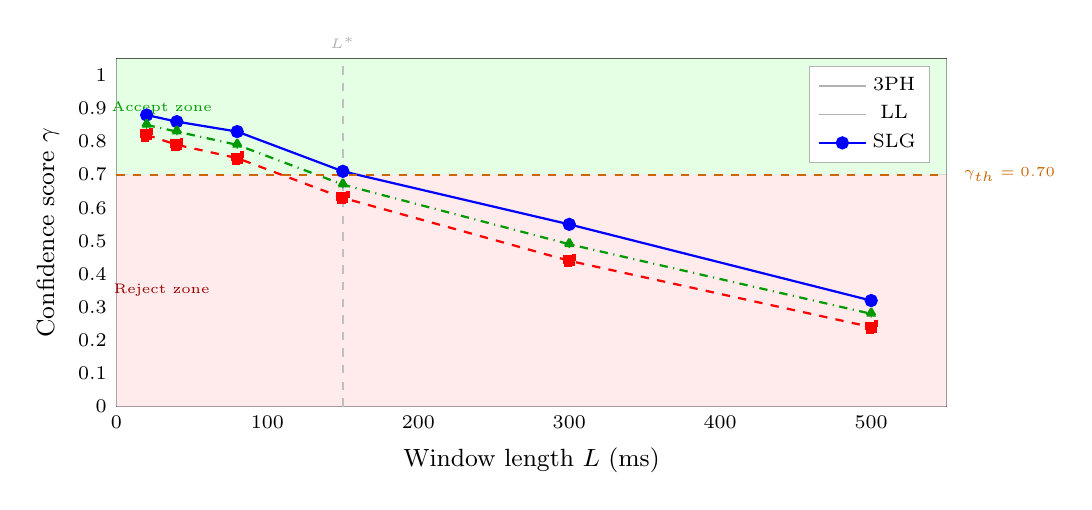
\begin{tikzpicture}
\begin{axis}[
  width=\columnwidth, height=6.0cm,
  xlabel={Window length $L$ (ms)},
  ylabel={Confidence score $\gamma$},
  xmin=0, xmax=550, ymin=0, ymax=1.05,
  xtick={0,100,200,300,400,500},
  ytick={0,0.1,0.2,0.3,0.4,0.5,0.6,0.7,0.8,0.9,1.0},
  ymajorgrids=true, grid style={gray!20},
  label style={font=\small},
  tick label style={font=\scriptsize},
  legend style={at={(0.98,0.98)}, anchor=north east,
                font=\scriptsize, fill=white, draw=black!30},
  clip=false
]

% Accept zone (γ > 0.70) — light green
\addplot[fill=green!10, draw=none]
  coordinates {(0,0.70)(550,0.70)(550,1.05)(0,1.05)} \closedcycle;

% Reject zone (γ < 0.70) — light red
\addplot[fill=red!8, draw=none]
  coordinates {(0,0)(550,0)(550,0.70)(0,0.70)} \closedcycle;

% Zone labels
\node[font=\tiny, green!60!black] at (axis cs:30, 0.90) {Accept zone};
\node[font=\tiny, red!60!black]   at (axis cs:30, 0.35) {Reject zone};

% 3PH
\addplot[blue, solid, thick, mark=*, mark size=2pt] coordinates {
  (20,0.88)(40,0.86)(80,0.83)(150,0.71)(300,0.55)(500,0.32)
};
% LL
\addplot[red, dashed, thick, mark=square*, mark size=2pt] coordinates {
  (20,0.82)(40,0.79)(80,0.75)(150,0.63)(300,0.44)(500,0.24)
};
% SLG
\addplot[green!60!black, dashdotted, thick, mark=triangle*, mark size=2pt] coordinates {
  (20,0.85)(40,0.83)(80,0.79)(150,0.67)(300,0.49)(500,0.28)
};

% Acceptance threshold
\draw[thick, orange!80!black, dashed]
     (axis cs:0, 0.70) -- (axis cs:550, 0.70);
\node[right, font=\tiny, orange!80!black]
     at (axis cs:555, 0.70) {$\gamma_{th}=0.70$};

% Validity boundary
\draw[thick, gray!50, dashed]
     (axis cs:150, 0) -- (axis cs:150, 1.05);
\node[above, font=\tiny, gray!60] at (axis cs:150, 1.05) {$L^*$};

\legend{3PH, LL, SLG};

\end{axis}
\end{tikzpicture}
